\chapter{ Cosmological simulations }


Currently in cosmology, one issue is to find the way
the dynamics of the Universe evolves from its first 
stages to the actual epoch. Computational resources 
appear as a necessary tool to tackle such problems
due to the big amount of interacting particles. 
If all possible components of the Universe would be considered 
in its evolution, the particles required to simulate 
the interaction among them would be so huge that it would not be viable
to predict the evolution of every single particle. Hence, numerical approximations 
must be developed to find for every time step all the properties needed to describe 
the system, even when particles studied have masses with magnitude order of several 
stellar masses. 

In cosmological simulations a key component to consider
is dark matter, since it is mostly because of this one that 
the Universe has a filament structure. 
The latter asseveration is due to dark matter dominates the gravitational
interaction, not only because of its amount compared to
baryonic matter but also because it only interacts in this way.

This component cannot be observed directly cause it does not interact 
with radiation. But, since its gravitational effects are strong, there are 
observational evidence that accounts for its existence. For example, 
observing galaxy rotation curves, the velocity measured at the outskirts 
of spiral galaxies was too fast to explain with only baryonic matter. 

Defining as total density the sum of baryonic and dark matter,
a key argument to ignore baryonic matter in simulations can be
given, dark matter would contribute with around $80\%$ of all 
this density content. Hence, the assumption that the Universe
dynamics is determined by dark matter is plausible.

The next chapter is divided in several sections, the first one
corresponds to the methods used in cosmological simulations to
calculate the gravitational evolution of the system. The second
one contains different criteria selection to detect a dark matter
halo in simulations. The third and fourth sections are dedicated
to explain how to build two different statistical measures of clustering
in real space, the correlation function and in fourier space, the power spectrum. 
The text books and articles that are used as reference in the next chapter
are \cite{Djeong}, \cite{Longair}, \cite{tree}, \cite{Klypin}, \cite{Klypin2},
\cite{Klypin3}, \cite{Jing}, \cite{Mont}.


%&&&&&&&&&&&&&&&&&&&&&&&&&&&&&&&&&&&&&&&&&&&&&&&&&&&&&&&&&&&&&&&&&&&&&&&&&&&&&&&&&&&&&&&&&&&&&&&&&&&&&&&&&&&&&&&&&&&&&&
\section{ Numerical methods }
%&&&&&&&&&&&&&&&&&&&&&&&&&&&&&&&&&&&&&&&&&&&&&&&&&&&&&&&&&&&&&&&&&&&&&&&&&&&&&&&&&&&&&&&&&&&&&&&&&&&&&&&&&&&&&&&&&&&&&&


To study the Universe evolution at big scales, simulations of dark matter
interacting particles inside a cosmological boxe are performed. 
In such cases is necessary to suppose initial conditions,
an initial configuration of the Universe, i.e., an initial density field
or an initial shape for the power spectrum. As mentioned, in these cosmological 
simulations dark matter is a key component, in many cases is the only particle considered.
Hence, it is important to provide some observational evidences encountered. 
As already stated dark matter does not interact with radiation, nevertheless it turns
out that the gravitational effects that causes are esential for the dynamical evolution
of the Universe. It is around the  $\sim 24\%$ content of the Universe.

One of the first observational evidence was found in the Coma cluster due to
a mass estimation from the virial theorem, let us see this in more detail: 
the specific kinetic energy of the system is $T = v^2/2 \sim 3\sigma^2/2 $ 
where $\sigma$ is the galaxy velocity dispertion and the potential energy
is $U = 3GM_{vir}/(5R_{vir})$. From the mass-luminosity ratio and the 
mean luminosity of the cluster, a second estimative of the mass is found. There is
such a big discrepancy between the two values that is reasonable to affirm that $\sim 90\%$ of the 
cluster's mass is not visible. 

The rotation curve of the galaxies can be other prove for dark matter existence,
for example, the velocity measures performed with respect to the radious of Andromeda 
galaxy (or another spiral galaxies) is approximately the same independent of the radial
distance of the stars to the center of the galaxy. From this, it could be affirmed that
density is uniform along the galaxy contrary to expected for the observed 
number of star in function of the radius. 


Another example is the Bullet cluster, composed by two two clusters that are colliding, 
an event not commonly observed. The gas of them reaches velocities around $\sim 10$ $millions$ $of$ $miles/h$ during the violent collision while they interact among them because of their charge. 
This interaction disminishes the gas velocity but this does not happen with dark
matter cause it does not interact electrically. 
Using gravitational lensing a distortion map is obtained. Using the X rays detected
and the distortion map, four different groups of matter are found, 2 bigger ones
that correspond to the dark matter component and two smaller ones that correspond
to luminous matter formed from the intercluster gas. These presents a strong
evidence of dark matter existence. 

\

So, additional to the initial conditions, the box size $L$ and the number of 
dark matter particles $N^3$ that would be used should be fixed. 
The gravitational interaction calculation of such a big number of particles
could in principle be calculated through direct sum of forces. This first
attempt is not very efficient or even it is not possible to perform
since the computing time or the computational resources would be very 
big to be viable. The latter is the reason for approximate methods 
to appear as a possible solution that implies more reasonable computing times.

A main objective in a simulation could be the study the formation process, fusion and
further interactions that are produced among halos and vacuum regions that conform
the filamentary structure of the Universe. Next, three of the most known numerical 
methods for cosmological simulations are going to be briefly exposed.

\begin{enumerate}
\item \textbf{Particle Mesh (PM)}\cite{tree}

In this method a grid is created over the particle array
as shown in the figure \ref{PM}. The particles more closed
to a vertice are assigned to this, to an specific cell, getting the density. 
Other way to calculate the density is cloud in cell, later explained
in more detail, where particles are considered constant density cubes causing
that a single particle contributes to different cells.
Using Poisson equation the potential in every grid vertice can be found
thanks to the Fourier transform. The potential calculation or the force of 
each particle can be interpolated among the points created by the 
grid. 

Although this method reduces considerably the computing time 
since its of the order of O($N+M\log M$) with $N$ being the number of particles
and $M$ the number of vertices. The lack of resolution in the regions that are
more dense makes this method insufficient to respond for the physical situation.
Furthermore, it does not give account for a complex geometry or systems
higly correlated. A step forward in this direction is $P^3M$ that uses
for smaller scales finer calculations making a particle particle calculation. 

%**********************************************************************************************************************
\begin{figure}[htbp]
       \centering
               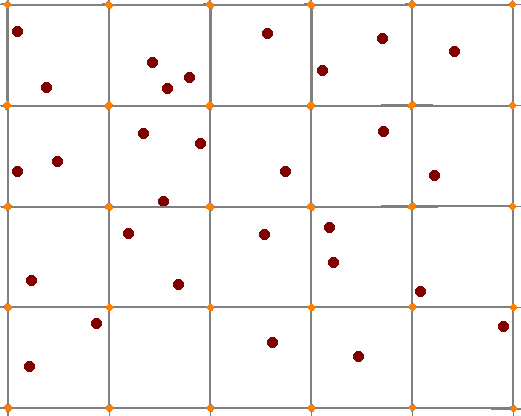
\includegraphics[width=0.35\textwidth]{Images/chapter3/MG.png}
       \caption{\small Particle mesh method. Every vertice of the grid gets 
       properties calculated from the closer particles.}
       \label{PM}
 \end{figure}
%**********************************************************************************************************************


\item \textbf{Tree method}\cite{tree}


To illustrate this method let us consider a 2D particle array. 
This square is divided in small cells of the same area where
each particle is assigned to a specific cell. 
If this number is superior to one, subdivisions of the cell
are performed and again if the number of particles per subcells 
is superior to one, subdivisions are made once more. This
process is repeated until for every cell there is at most
one particle. 
This subdivision is used to create a tree structure, this consists
in a root, i.e., all the square area and the branches that are 
created with each subdivision performed. This serves as a map
of the disposition of the particles in the square array. 
The particles are numerate from the upper left of the square 
until all particles in the first cell are numerate following with
the second cell until the lower left is reached. 

When the gravitational calculation is performed, the contribution 
to the force exerted over a particle due to the more distant ones
is much lower than with the nearer. Hence, the far ones can be 
approximated as a seudoparticle with mass $M$ and with a position
$r_{CM}=\sum_im_ir_i/M$. As a selection criteria the next expression
is taken

\begin{equation}
s/q\leq \theta
\label{sq}
\end{equation}

where $s$ is the cell size with wich the particle of interest is interacting 
with, $d$ the distance cell partilce and $\theta$ is a tolerance value to
define. When the condition is satisfied the gravitational interaction 
is calculated directly with the seudoparticle. In the opposite case the 
relation \ref{sq} for the subcells that contain the studied cell and that way
successively until the condition is satisfied or only one particle is 
present per cell. In this way the direct calculation is avoided for far
objects without avoiding the calculation for the nearer ones. 
Therefore, the computing time is reduced from $O(N^2)$ to $O(N\log(N))$.

%**********************************************************************************************************************
\begin{figure}[htbp]
       \centering
               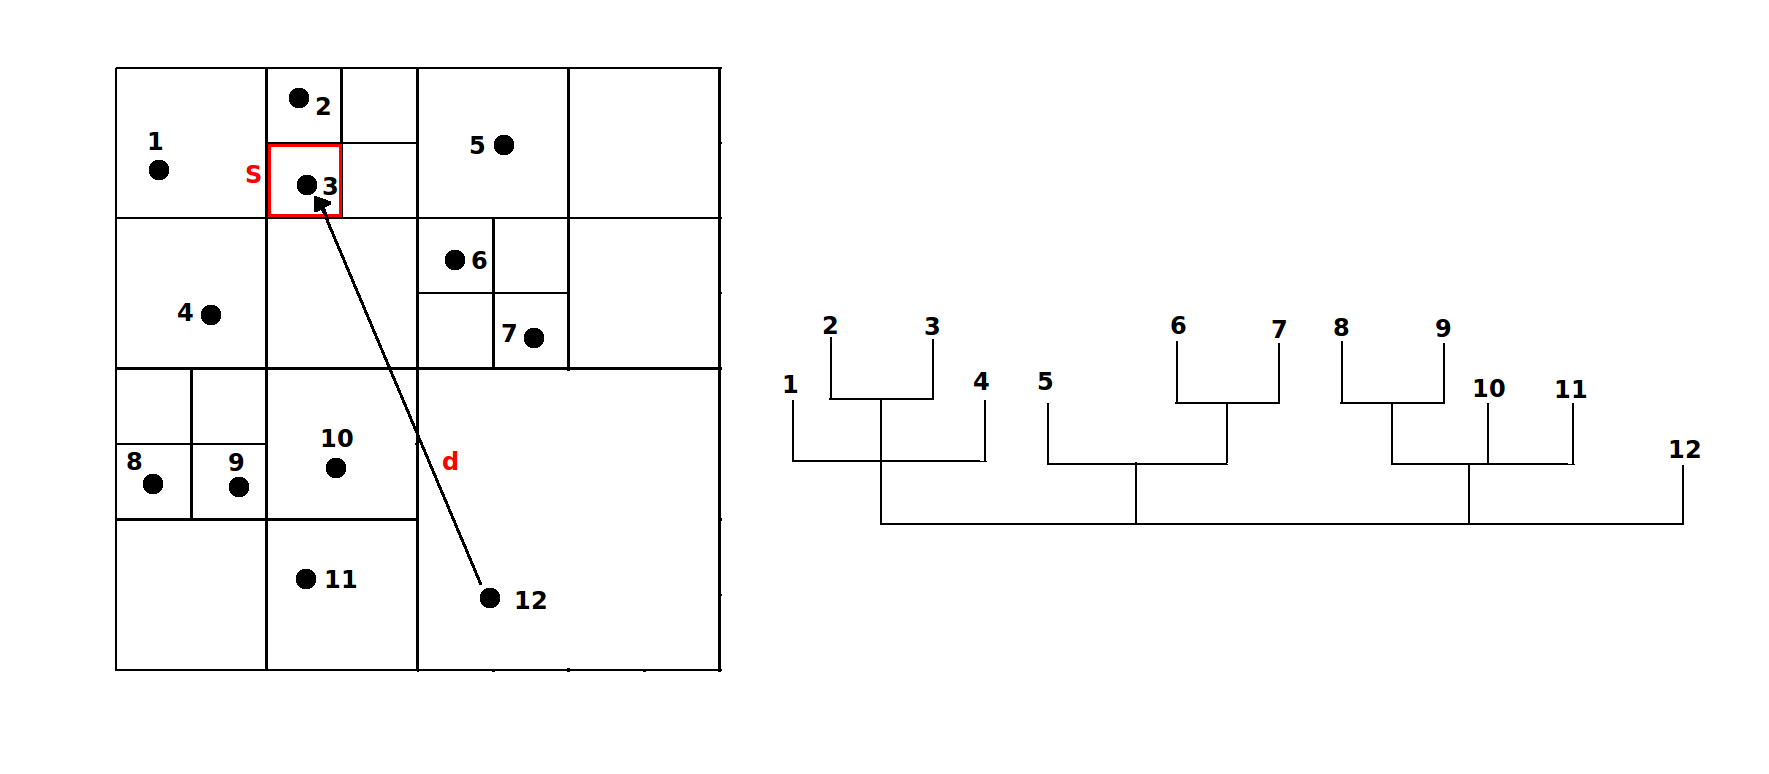
\includegraphics[width=1.0\textwidth]{Images/chapter3/treecode.png}
       \caption{\small In the left panel is shown the array of the particles and the subdivisions performed until at most one particle is found per cell. In the right one, the tree found for such distribution is shown.}
       \label{tree}
 \end{figure}
%**********************************************************************************************************************


\item ART Code\cite{klypin}

As its acronym indicates, Adaptive Refinement Tree Code consists in a multigrid
code. An initial grid is created where the Poisson equation is solved afterwards
followed by a refinement according to overdensities that are in certain regions.
Even after performing the refinement over the grid, this calculation can be 
continously being performed. Here, calculations particle particle are not being
performed. Something new compared to the methods previously exposed is that 
the cell shape can take any form allowing to get an adaptive grid depending on
the amount of particles in the region. 

\end{enumerate}

There are many methods that are hibrid among the 3 exposed, for example 
the already mentioned $P^3M$. All of them have both advantages and disadvantages
that need to be evaluated according to the needs of the simulation. 

\

%&&&&&&&&&&&&&&&&&&&&&&&&&&&&&&&&&&&&&&&&&&&&&&&&&&&&&&&&&&&&&&&&&&&&&&&&&&&&&&&&&&&&&&&&&&&&&&&&&&&&&&&&&&&&&&&&&&&&&&
\section{ Halo selection }
%&&&&&&&&&&&&&&&&&&&&&&&&&&&&&&&&&&&&&&&&&&&&&&&&&&&&&&&&&&&&&&&&&&&&&&&&&&&&&&&&&&&&&&&&&&&&&&&&&&&&&&&&&&&&&&&&&&&&&&

As a result of the dark matter particle interactions, perturbations 
grow enough to form ligated objects hence they are in virial equilibrium,
these are known as dark matter halos and satisfy $E_k=-V/2$. 
They are responsible for the potential wells that causes baryonic matter 
to fall in, finally forming the galaxies we observe today, i.e., dark
matter halos host galaxies. 

A main result of a cosmological simulation are the dark matter halos 
catalogue, which we are going to work with, that contains halo properties such
as position, velocity, mass, radious and redshift. Thus, a key step is to identify 
halos from a cosmological simulation, the methods generally use to acomplish such 
task are FOF and BDM 

\begin{enumerate}

%######################################################################################################################
\subsection{ Friends of friends }
%######################################################################################################################

\item Friend of Friends (FOF) 

To identify if a particles group lies in a dark matter halo, i.e., particles 
are linked, a length is defined such that all the particles that lie inside 
are part of the same group. This distance is called linking length. A condition 
is imposed, groups can not intersect among them, hence a particle can only belong 
to a specific group. But there is a problem with this approach, even when there is 
a little amount of particles in common between two groups, some sort of small 
``bridge`` that unites both of them, they are selected as one group not two
as would be expected. This method also allows to define substructures, therefore using
different linking lengths groups inside groups would be obtained, the bigger ones
would host the smaller ones. 

%######################################################################################################################
\subsection{ Bound density maximum }
%######################################################################################################################

\item Bound Density Maximun(BDM)

For this method the local maximum densities in the particle array of the simulation
are detected. From them a spherical cut is defined and the particles inside form 
the dark matter halo. Particles with bigger or equal velocity than the scape one
are not included in the halo. 
Contrary to FOF method, halos can overlap while the center of mass of one halo 
does not fall into the other one. Nevertheless, if the center of mass of one halo
fall in the virial radious of other one, this is considered a subhalo of the last
one. The standard overdensity limit of the halos is $360\rho_{back}$ where $\rho_{back}$
is the background density. 

\end{enumerate}

%&&&&&&&&&&&&&&&&&&&&&&&&&&&&&&&&&&&&&&&&&&&&&&&&&&&&&&&&&&&&&&&&&&&&&&&&&&&&&&&&&&&&&&&&&&&&&&&&&&&&&&&&&&&&&&&&&&&&&&
\section{Density field in a cosmological simulation}
%&&&&&&&&&&&&&&&&&&&&&&&&&&&&&&&&&&&&&&&&&&&&&&&&&&&&&&&&&&&&&&&&&&&&&&&&&&&&&&&&&&&&&&&&&&&&&&&&&&&&&&&&&&&&&&&&&&&&&&

To construct a good approximation of the real density field from a cosmological simulation, 
a sampling of the continuous density field in a regular grid of size $N^3$ is 
performed, the subdivisions created are called cells. Hence, an assignment of the 
particle charge, i.e. particle mas, to the grid must be done. To obtain a more realistic 
density field approximation the grid points can be increased also disminishing problems 
due to numerical effects but it is more expensive computationally. Furthermore, the number 
of particles in a simulation is a restriction to the maximum value that $N$ can have, 
it can not exceed $\sqrt[3]{N_p}$, there would not be enough particles to map correctly 
the density field per cell. A size grid around the value mentioned would optimal in 
the sense that the particle mean per cell would be one, hence a Poisson distribution 
would be followed. But the sampling made from the particle distribution is not a 
mere sampling but a sampling convolved with a window function (the way a particle 
mass is distributed in the grid), i.e., the window function $W$ that is used affects 
the density field calculated. 

Since the particles are located in a specific position it can be assured that
the particle number density is 

\[n_0(\textbf{x}) = \sum_{i=1}^{N_{p}} \delta^D ( \textbf{x} - \textbf{x}_i )\]

where $\textbf{x}_i$ the position of the $i$-th particle. The window function 
quantifies how much of the particle number density is distributed to a grid point 
separated by $\textbf{x}$, hence the sample particle number density can expressed as 

\[n(\textbf{x}_p) = \int_V d^3 x' n_0(\textbf{x'}) W(\textbf{x}_p-\textbf{x'})\]

Similarly, the sampled density contrast defined as $\delta^s(\textbf{x})=n(\textbf{x}_p)/\bar{n}-1$ 
can be found using the convolution of the real density contrast and the window function 

\begin{equation}
\delta^s(\textbf{x}) = [\delta*W](\textbf{x})
\label{df_conv}
\end{equation}

its fourier transformation is simply the product of the fourier transformation of the real 
density contrast and the window function 

\begin{equation}
\delta^s(\textbf{k}) = \delta(\textbf{k})W(\textbf{k})
\label{df_four}
\end{equation}

thus, the real density contrast can be obtained dividing the sampled density contrast with
the window function used. 

\

The procedure of convolving with a window function can be seen in a different way, if a 
point spreading or cloud shape function $S(x')$, being $x'$ the distance from the particle
position $x_i$, is carried by each particle then the charge assigned to the grid point $x_p$ 
is given by the overlap of the shape function within the cubic cell $p$

\[W(x)=\int \Pi \left(\frac{x'}{H} \right) S(x'-x)dx' \]

where $\Pi(x)$ is the top hot function and $H=L/N$ is the size of a cell. 

There are 3 commonly used schemes for the mass assignment, nearest grid point, cloud
in cell and triangular shaped cloud. For each case we are going to consider a one dimensional
window function. The sencond and third one are first and second order distribution schemes
respectively, hence each of them is a better approximation than the previous one. 

\

\textbf{Nearest grid point: } The first scheme considers that the particle charge is 
assigned to the cell where the particle falls, each cell is centered 
in a grid point, therefore the particle is assigned to the nearest grid point. 
Let us see this in more detail. If the cloud shape interpretation is used, the particle 
shape would be a Dirac delta function that would be assigned to the specific cell 
where particle falls in as shown in the figure \ref{NGP} (a). If the other interpretation 
is considered, the window function would be a top hat function centered in the particle, 
the value assigned to grid point would the one that top hat function would get when is 
evaluated in that grid point as shown in figure \ref{NGP} (b). 

\begin{eqnarray*}
 W_{NGP}(x)  =  \Pi \left( \frac{x}{H} \right) & \equiv & \frac{1}{H}\Pi\left(\frac{x}{H}\right) *\delta \left(\frac{x}{H}\right) \\ 
&  = &\frac{1}{H}\Pi\left(\frac{x}{H}\right)*S\left(\frac{x}{H}\right)
\end{eqnarray*}

This window function in the fourier space is

\[ W_{NGP}(k)= sinc\left(\frac{\pi k}{2k_N} \right)\]

where $k_N$ is the Nyquist frequency that later will be defined. 

%**********************************************************************************************************************
\begin{figure}[htbp]
       \centering
               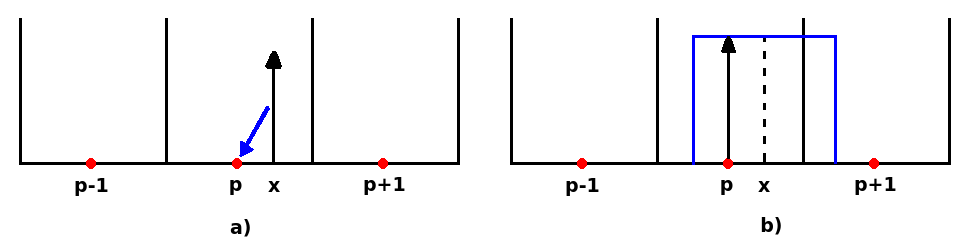
\includegraphics[width=0.8\textwidth]{Images/chapter3/NGP.png}
       \caption{\small The left figure shows the cloud shape interpretation where the Dirac function
       is assigned to the particle grid. The right one shows the window function interpretation
       where the top hat function evaluated in the grid point would give the charge assigned to it. }
       \label{NGP}
 \end{figure}
%**********************************************************************************************************************

\textbf{Cloud in cell: } This scheme assumes that the charge of a specific particle 
assigned to a grid point is given by the overlap of a cell with a size H centered in 
the particle with the cell centered any the grid point. Then, the particle not only 
contributes to the cell where it falls in but also to some of the 26 neighbour cells. 
This explanation is shown in the left figure of \ref{CIC} but according to the window 
function explanation, a ''triangle'' function $\Lambda(x)$ centered in the particle and length
H is evaluated in the corresponding grid points of the cells, the one where particle falls 
in and the neighbour ones, finding the contribution of the charge to every one of them
as shown in figure  \ref{CIC} (b).  

\begin{eqnarray*}
 W_{CIC}(x)  =  \Lambda \left( \frac{x}{H} \right) & \equiv & \frac{1}{H}\Pi\left(\frac{x}{H}\right) *\Pi \left(\frac{x}{H}\right) \\ 
&  = &\frac{1}{H}\Pi\left(\frac{x}{H}\right)*S\left(\frac{x}{H}\right)
\end{eqnarray*}

This window function in the Fourier space is

\[ W_{CIC}(k)= sinc^2\left(\frac{\pi k}{2k_N} \right)\]

hence, the Fourier transform of the CIC window function is the square of the Fourier 
transform of the NGP window function. 

%**********************************************************************************************************************
\begin{figure}[htbp]
       \centering
               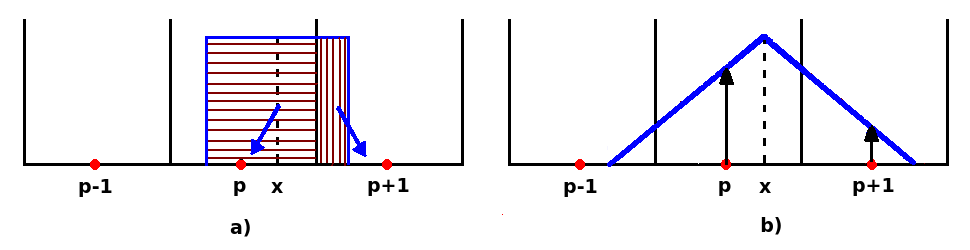
\includegraphics[width=0.8\textwidth]{Images/chapter3/CIC.png}
       \caption{\small The left panel shows the CIC cloud shape function and the intersection
       between the cell centered in the particle with the cells provides the contribution of
       the charge to every cell. The right one shows a ''triangle''	 function that is evaluated
       in every grid point to find the charge contribution to the cell. }
       \label{CIC}
 \end{figure}
%**********************************************************************************************************************

\textbf{Triangular shaped cloud: } This scheme is as the two previously presented but the cloud
shape function and the window function changes. As it happens with CIC, TSC contributes to diffent
cells, not only the one where it falls in. Both interpretations are shown in the figure \ref{TSC}.
Next the expression to calculate the charge contribution to a specific cell is given by

\begin{eqnarray*}
 W_{TSC}(x)  &=& \frac{1}{H}\Lambda \left( \frac{x}{H} \right)*\Pi \left(\frac{x}{H}\right) \\ 
&  = &\frac{1}{H}\Pi\left(\frac{x}{H}\right)*S\left(\frac{x}{H}\right)
\end{eqnarray*}

The Fourier transform of the window function is 

\[ W_{TSC}(k)= sinc^3\left(\frac{\pi k}{2k_N} \right)\]

hence, the Fourier transform of the TSC window function is the cubic of the Fourier 
transform of the NGP window function. 

%**********************************************************************************************************************
\begin{figure}[htbp]
       \centering
               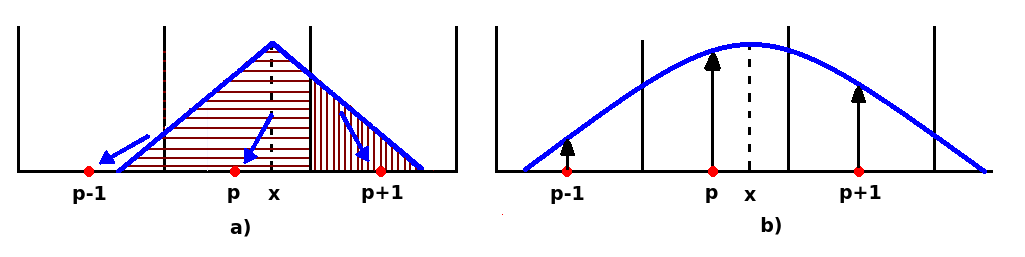
\includegraphics[width=0.8\textwidth]{Images/chapter3/TSC.png}
       \caption{\small The left figure shows the cloud shape function, a ''triangle'' function
       and the overlap with the cells provides the value of the charge assigned to every cell. But
       using the window function interpretation the right figure is obtained, where the particle carries
       with a function that evaluated in every grid point gives the contribution to the specific cell. }
       \label{TSC}
 \end{figure}
%**********************************************************************************************************************

\

Hence, each successively higher order assignment function is obtained by convolving the previous
assignment function with $\frac{1}{H}\Pi\left(\frac{x}{H}\right)$. 

From a one dimensional window function can be obtained the three dimensional one, simply as
the multiplication of the three one dimensional ones. This last asseveration is valid due to 
the grid used is regular. 

Thus, for every cell contained in the cosmological box a value of the convolved density 
field is calculated using a specific mass assignment scheme. 

%&&&&&&&&&&&&&&&&&&&&&&&&&&&&&&&&&&&&&&&&&&&&&&&&&&&&&&&&&&&&&&&&&&&&&&&&&&&&&&&&&&&&&&&&&&&&&&&&&&&&&&&&&&&&&&&&&&&&&&
\section{ Power spectrum in cosmological simulations }
%&&&&&&&&&&&&&&&&&&&&&&&&&&&&&&&&&&&&&&&&&&&&&&&&&&&&&&&&&&&&&&&&&&&&&&&&&&&&&&&&&&&&&&&&&&&&&&&&&&&&&&&&&&&&&&&&&&&&&&


The density perturbations of the ensemble, convolved density field for every cell 
of the box, allow to calculate the power spectrum as shown in equation \ref{pk},
an esemble average for every mode $\kappa$. Since this a statistical measure in
the Fourier space let us see the Fourier transform in more detail.

\subsection{Fourier transform}

The fourier transform is defined for this work with the next convention

\begin{equation}
F(\boldsymbol{\kappa}) = \int_{-\infty}^{\infty} d^3 x f(\textbf{x})e^{-i \boldsymbol{\kappa}\cdot\bf{x}	}
\label{FT}
\end{equation}

with $\kappa$ being the wave number vector. The inverse fourier transform as

\begin{equation}
f( \boldsymbol{x}) = \int_{-\infty}^{\infty} \frac{d^3 \kappa}{(2\pi)^3}  F(\boldsymbol{\kappa})e^{i \boldsymbol{\kappa}\cdot\bf{x}	}
\label{IFT}
\end{equation}

The convolution of the functions $g(\bf{x})$ and $f(\bf{x})$ is defined as follows

\[h(\bf{x}) = |g*f|(\bf{x})\equiv \int_{-\infty}^{\infty} g(\bf{x}')f(\bf{x} - \bf{x}') d^3 x' \]

but the Fourier transform of $h(\bf{x})$ is 

\[H(\boldsymbol{\kappa}) = G(\boldsymbol{\kappa}) F(\boldsymbol{\kappa})  \]

this is known as the convolution theorem. It is used in our work since the fourier 
transform of the window function convolved with the density field (equation \ref{df_conv})
allow us to obtain the real density field. From equation \ref{df_four} 

\[\delta(\textbf{k}) = \delta^s(\textbf{k})/W(\textbf{k})\]

In the situation we are dealing with, the function $F(\boldsymbol{\kappa})$ is only
sampled at evenly spaced intervals ($N^3$ frequencies totally) since we only 
know $f(\textbf{x})$ in $N^3$ points

\begin{eqnarray*}
F(\boldsymbol{\kappa}) =\left\{ \begin{array}{cl}
F(\kappa_F\boldsymbol{n}_\kappa) \hspace{1em} & \boldsymbol{n}_\kappa = (i,j,k) \in Z^3\\
0 \hspace{1em} & \mathrm{otherwise}\\
\end{array}\right.
\end{eqnarray*} 

where $\kappa_F=2\pi/L$ is the fundamental frequency.

Due to the functions are only sampled in specific points, the integrals defined in 
equations \ref{FT} and \ref{IFT} can be approximated to the discrete Fourier transform. 
Let us express them in terms of the density fluctuations in real and Fourier space 
because they are the ones of interest for our work 

\begin{eqnarray*}
\delta(\boldsymbol{\kappa}_p) = H^3 \sum_{n_p} \delta(\boldsymbol{r}_p) e^{-i\boldsymbol{\kappa}_p\cdot \boldsymbol{x}_p} \\
\delta(\boldsymbol{r}_p) = \frac{1}{L^3}\sum_{\boldsymbol{k}_p} \delta(\boldsymbol{\kappa}_p) e^{i\boldsymbol{\kappa}_p\cdot \boldsymbol{x_p}} 
\end{eqnarray*} 

where $H = L/N$ is the separation of the grid in the real space, 
$\boldsymbol{\kappa}_p = k_F \textbf{n}_p$ and $ \boldsymbol{n}_p = (i,j,k)$ with each index
varying from $-N/2 \leq i,j,k \leq N/2$ . The function $\delta(\boldsymbol{r}_p)$  is sampled 
in the points $\boldsymbol{r}_p$ and $\delta(\boldsymbol{\kappa}_p)$ in the points 
$\boldsymbol{\kappa}_p$. Therefore, the Fourier space is divided into small cells, N cubes of size 
$\kappa_g = 2\pi/H$ per dimension as it was done for the simulation. 

Furthermore, the extreme values for $\boldsymbol{n}_p$ correspond to Nyquist critical 
frequency 

\[\kappa_N = \pi\frac{N}{L} = \frac{\pi}{H} \]

thus, $-\kappa_N < k < \kappa_N $. A phenomenon called aliasing appears when a continuous 
function is sampled and is not bandwidth limited to a frequency smaller than $\kappa_N$. 
It consists in a folding over or aliasing of the frequencies that fall outside the range
as shown in figure \ref{alias}. 

%**********************************************************************************************************************
\begin{figure}[htbp]
       \centering
               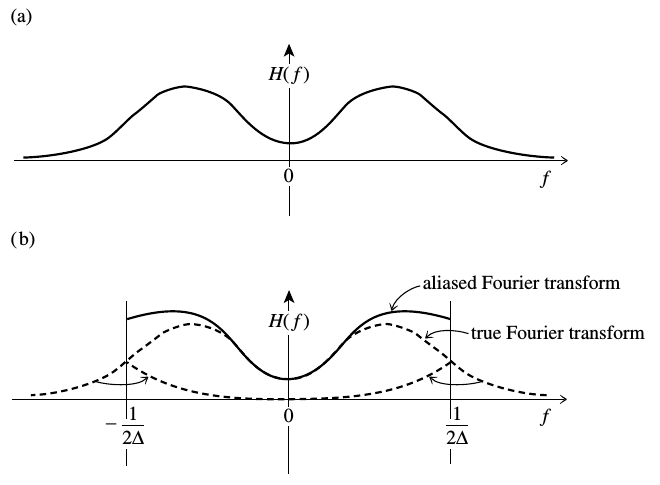
\includegraphics[width=0.8\textwidth]{Images/chapter3/aliasing.png}
       \caption{\small Aliasing effect for $H(f)$ sampled with a space interval $\Delta$.
       Frequencies outside the frequency range are included into the range because
       of the discrete sampling of the function. Figure taken from \cite{Press}.}
       \label{alias}
 \end{figure}
%**********************************************************************************************************************

To perform the discrete Fourier transform of the sampled density field was used the free 
library FFTW, where a fast Fourier discrete transformation (FFT) is implemented.
Because of algorithmic details of the FFT the fourier coefficients are ordered in the
following manner

\begin{eqnarray*}
\kappa_l(i) =\left\{ \begin{array}{cl}
\frac{2\pi}{L}i \hspace{1em} & \mathrm{if} \hspace{1em} i = 0,\dots ,\frac{N}{2}\\
\frac{2\pi}{L}(-N+i) \hspace{1em} & \mathrm{if} \hspace{1em} i = \frac{N}{2}+1,\dots ,N-1\\
\end{array}\right.
\end{eqnarray*} 


where the subindex $l$ stands for $x,y$ or $z$ coordinate. 
The library has different routines, one is a complex to complex function, this is, perfoms a 
Fourier transformation of a sampled complex function. Other one, named real to complex routine, 
takes the real samples of a function to find the Fourier transformation. The last one 
uses the Hermitian condition that allows to improve the calculation in speed and memory 
usage

\[\delta_\kappa(-\textbf{n}_\kappa) = \delta_\kappa^*(\textbf{n}_\kappa)\]

where the superscript $*$ denotes complex conjugate. In both cases a normalization 
must be taken into consideration, this can be noticed in the relation between the transformed 
density field obtained with FFTW and the sampled space density field 

\[\delta^{FFTW}(\textbf{n}_k) = \sum_{r_p} \delta(\textbf{r}_p)e^{-i\boldsymbol{\kappa}_p\cdot \boldsymbol{r}_p} = \frac{\delta(\boldsymbol{\kappa}_p)}{H^3}\]

with the last expression and the definition of PS given in equation \ref{pk}, the power
spectrum from FFTW is given by \cite{Djeong}

\begin{equation}
P(\kappa_F n_1) = \frac{H^6 k^3_F}{(2\pi)^3}\langle\delta^{FFTW}(\mbox{\boldmath$n$}_1\delta^{FFTW}(-\mbox{\boldmath$n$}_1)\rangle = \frac{V}{N^6}\langle|\delta^{FFTW}(\mbox{\boldmath$n$}_1)|^2\rangle
\end{equation} 

this is the power spectrum estimator that is used throughout this work. 

\subsection{PS calculation}

To calculate the power spectrum, the next steps are followed

\begin{enumerate}

\item[1)] From a cosmological box of size L, a grid with $N^3$ subdivisions is performed
creating cells of volume $H^3$. 

\item[2)] The sampled space density field is created using a specific window function,
mass of particles are assigned to the grid. 

\item[3)] With FFTW software, the FT of the sampled space density field is calculated.

\item[4)] To deconvolve and eliminate the aliasing effect $P(\boldsymbol{\kappa})\equiv |\delta(\kappa)|^2$ is divided by the next window function, at each grid point or equivalently each cell

\[ W(\boldsymbol{\kappa}) = \prod^{3}_{i=1}\left[ 1 - \frac{2}{3}\sin^2\left(\frac{\pi\kappa_i}{2\kappa_N}\right) \right] \]

where $\boldsymbol{\kappa} = (\kappa_x,\kappa_y,\kappa_z)$ as proposed in \cite{Jeong}.  

\item[5)] The amount $P(\kappa)$ is calculated taking the spherical average of 
$P(\boldsymbol{\kappa})$ corrected inside the shell 
$\kappa -\Delta\kappa/2	< |\boldsymbol{\kappa}|<\kappa +\Delta\kappa/2$.

\end{enumerate}


%&&&&&&&&&&&&&&&&&&&&&&&&&&&&&&&&&&&&&&&&&&&&&&&&&&&&&&&&&&&&&&&&&&&&&&&&&&&&&&&&&&&&&&&&&&&&&&&&&&&&&&&&&&&&&&&&&&&&&&
\section{ Correlation functions in cosmological simulations }
%&&&&&&&&&&&&&&&&&&&&&&&&&&&&&&&&&&&&&&&&&&&&&&&&&&&&&&&&&&&&&&&&&&&&&&&&&&&&&&&&&&&&&&&&&&&&&&&&&&&&&&&&&&&&&&&&&&&&&&


In practice, to calculate in a cosmological simulation the correlation function 
a at distance $r$, it has to be performed an average of the number of neighbours per 
particle at a given scale or the binned comoving separation. In this direction 
correlation function estimators can be used, one of the most basic ones is shown below. 
Two catalogues are considered for this estimator, one is our particles box, 
data-data catalogue (DD) and the second one is generated 
randomly with at least the same number of particles and the same size of the box, 
random-random catalogue (RR). The DD catalogue should have regions with more or
less clustering than a homogeneous distribution, this is precisely the RR catalogue role, 
a way to measure how much the DD catalogue deviates from the homogenous distribution. 

From this estimator is easier to notice that $\xi(r)$ is a measure of 
excess or deficiency of clustering at $r$ making it more intuitive 

\[1+\xi(r)= \f{\eta_{DD}(r)}{\eta_{RR}(r)}\]

here $\eta_{RR}(r)$ is the number of pairs of particles at a distance $r$ in the catalogue DD 
and $\eta_{RR}(r)$ is the number of pairs of particles at a distance $r$ in the catalogue RR. 

Other common estimators also need an additional catalogue, the data-random, where the
pair of particles would not only include the DD or RR but a mixed catalogue containing 
both arrays, making more robust the estimator proposed \cite{Est_CF}

\begin{eqnarray}
\mbox{Landy-Szalay Estimator}\hspace{0.5cm} \xi_{LS}(r)&=& 1+\frac{DD(r)}{RR(r)}\left(\frac{N_R}{N}\right)^2-2\f{DR(r)}{RR(r)}\left(\frac{N_R}{N}\right) \nonumber \\
\mbox{Hamilton Estimator}  \hspace{0.5cm} \xi_{HAM}(r)&=&\frac{DD(r)RR(r)}{DR(r)^2}-1 \nonumber 
\end{eqnarray}

where $N_R$ is the number of points of the RR catalogue and $N$ of the DD catalogue.

\subsection{Correlation function calculation}

To calculate the correlation function the Landy-Szalay estimator is used, the next
rough steps are followed to calculate it

\begin{enumerate}

\item[1)] A catalogue of $N_R$ particles is generated randomly in a cubic box of size L.

\item[2)] For a bin around $r$ the pair of galaxies in the DD, RR and DR catalogues are found
and using Landy-Szalay estimator the correlation function is found for that scale. 

\end{enumerate}